\chapter{Das Peugeot-Unfallauto}
Um den \textsc{Detroit} batterietechnisch auf den aktuellsten Stand zu bringen, sollten aus einem Unfallauto die Batterie sowie die dazugehörigen Bauteile entnommen werden. Beim Unfallauto handelt es sich um einen Peugeot Ion. Dieses Kapitel soll zum einen aufzeigen, wie der Peugeot funktioniert, da dessen Funktionsweise sich stark von der des \textsc{Detroits} unterscheidet. Zum anderen soll ebenfalls aufgezeigt werden, welche Bauteile aus welchen Gründen für den {Detroit} übernommen oder nicht übernommen wurden.

\section{Batterie}
Beim Peugeot lag das Hauptaugenmerk auf der Batterie. Diese war aufgebaut aus insgesamt 22 Viererblöcken vom Typ LEV50-4 \cite{lev50}. Jede Einzelzelle verfügt dabei über eine Kapazität von $50$ Ah bei einer Nennspannung von $3.7$ V. Da alle Zellen in Serie geschaltet waren, ergab sich eine Gesamtspannung von $22\cdot 4\cdot 3.7$ V$=325.6$ V. Zusammen mit der gleich gebliebenen Kapazität ergibt sich ein theoretischer Energiegehalt der Batterie von $325.6$ V$\cdot50$ Ah$=16.28$ kWh.

Auf jedem solchen Viererblock befand sich eine Sensorplatine des Batteriemanagementsystemes. Bereits auf dieser Platine wurden die Spannung sowie die Temperatur der einzelnen Zellen ausgewertet. Auch Balancierströme (dies sind Ströme, die die Spannungen der Einzelzellen angleichen) konnten auf diesen Platinen aktiviert werden. Eine solche Platine ist in Abbildung \ref{fig:BMS_Alt} zu sehen:

\begin{figure}[h!]
	\centering
		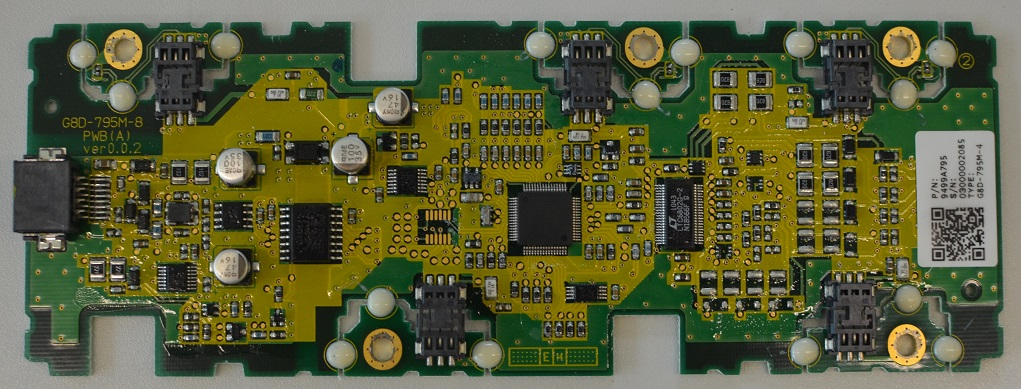
\includegraphics[width=0.80\textwidth]{images/BMS_Alt.JPG}
	\caption{Im Peugeot verbaute BMS-Sensorplatine}
	\label{fig:BMS_Alt}
\end{figure}

Die so gesammelten Daten wurden über eine proprietäre Verbindung an das Steuergerät übertragen, welches die Aufgabe hatte, die ausgewerteten Daten zu überwachen und gegebenenfalls Balancierströme oder weitere Schutzfunktionen zu schalten.

Da es nicht möglich war, auf die so gesammelten Daten zuzugreifen, musste dieser Teil der Batterie ersetzt werden und es konnten nur die Zellen ohne BMS übernommen werden.


\newpage